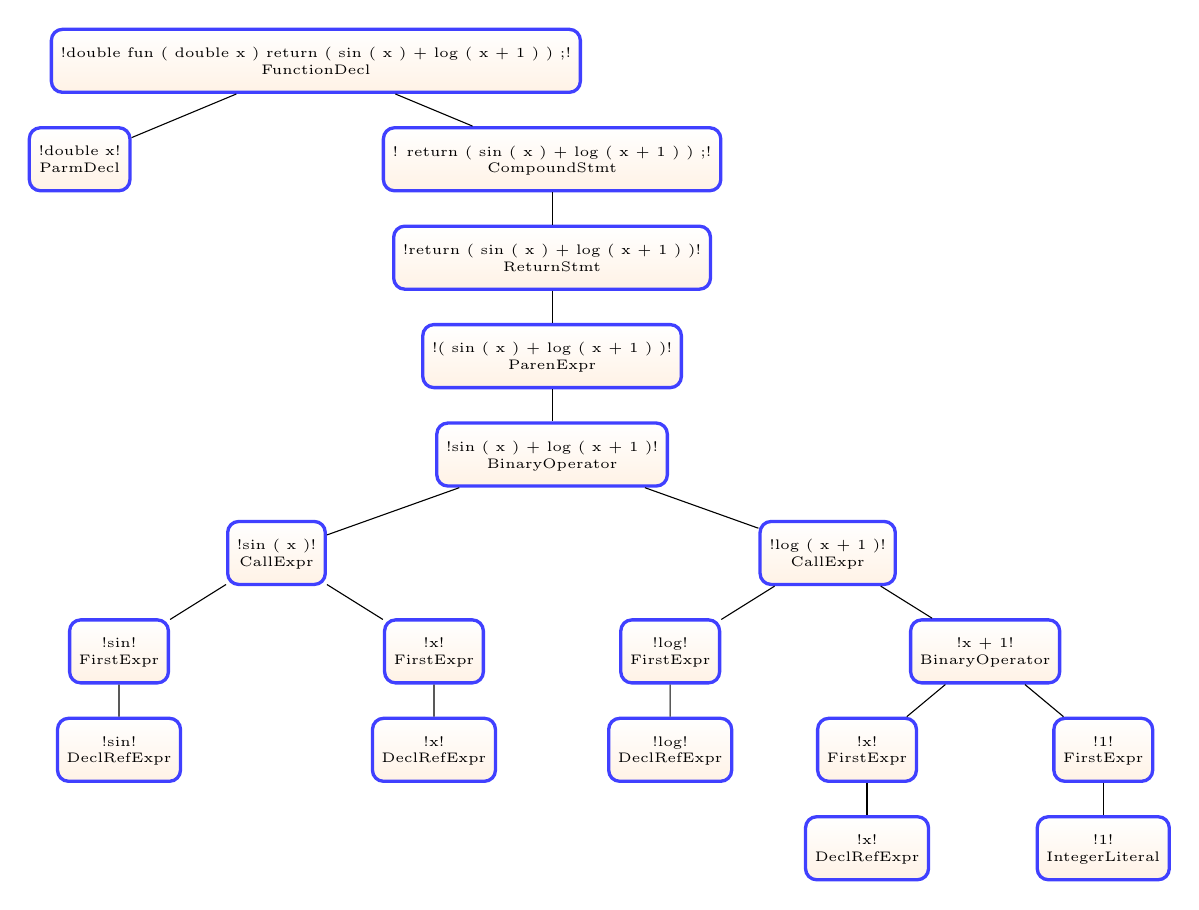
\begin{tikzpicture}
[
font=\tiny,
level distance=1.25cm,
level distance=1.25cm,
every node/.style={
    top color=white,
    bottom color=orange!10,
%    bottom color=blue!25,
    rectangle,rounded corners,
    minimum height=8mm,
    draw=blue!75,
    very thick,
%    drop shadow,
    align=center,
    text depth = 0pt},
 level/.style={sibling distance=6cm},
 level 4/.style={sibling distance=7cm},
 level 5/.style={sibling distance=7cm},
 level 6/.style={sibling distance=4cm},
 level 7/.style={sibling distance=3cm}
]
 \node {\Verb!double fun ( double x )  return ( sin ( x ) + log ( x + 1 ) ) ;!\\ FunctionDecl}
 child {
  node {\Verb!double x!\\ ParmDecl}
 }
 child {
  node {\Verb! return ( sin ( x ) + log ( x + 1 ) ) ;!\\ CompoundStmt}
  child {
   node {\Verb!return ( sin ( x ) + log ( x + 1 ) )!\\ ReturnStmt}
   child {
    node {\Verb!( sin ( x ) + log ( x + 1 ) )!\\ ParenExpr}
    child {
     node {\Verb!sin ( x ) + log ( x + 1 )!\\ BinaryOperator}
     child {
      node {\Verb!sin ( x )!\\ CallExpr}
      child {
       node {\Verb!sin!\\ FirstExpr}
       child {
        node {\Verb!sin!\\ DeclRefExpr}
       }
      }
      child {
       node {\Verb!x!\\ FirstExpr}
       child {
        node {\Verb!x!\\ DeclRefExpr}
       }
      }
     }
     child {
      node {\Verb!log ( x + 1 )!\\ CallExpr}
      child {
       node {\Verb!log!\\ FirstExpr}
       child {
        node {\Verb!log!\\ DeclRefExpr}
       }
      }
      child {
       node {\Verb!x + 1!\\ BinaryOperator}
       child {
        node {\Verb!x!\\ FirstExpr}
        child {
         node {\Verb!x!\\ DeclRefExpr}
        }
       }
       child {
        node {\Verb!1!\\ FirstExpr}
        child {
         node {\Verb!1!\\ IntegerLiteral}
        }
       }
      }
     }
    }
   }
  }
 }
;
\end{tikzpicture}
